\documentclass[a4paper,12pt]{report}
\usepackage[utf8]{inputenc}
\usepackage{graphicx}
\usepackage[margin=1in]{geometry}
\usepackage{setspace}
\usepackage{amsmath}
\usepackage{caption}
\usepackage{subcaption}
%\usepackage{titlesec}


\begin{document}
\setcounter{chapter}{1}
\chapter{Creating a Simple Geomtery in OpenFoam}
\flushleft\textbf{Introduction}
\flushleft In this chapter we will learn how to create a simple geometry and mesh it. Here we will use the lid-driven cavity problem example, mentioned in the previous chapter for pre-processing.  As previously mentioned you can type the following path in the command terminal to open the id-driven cavity problem$:$
\flushleft \textbf{cd OpenFOAM/OpenFOAM-2.3.0/run/tutorials/incompressible/icoFoam/cavity}
\flushleft After this if you type “ls” in the command terminal would see three folder inside it given as$:$

\begin{itemize}
\item 0
\item constant
\item system
\end{itemize}

\flushleft where the 0 folder gives the initial boundary conditions for that particular geometry, constant gives the geomtery file and other fluid properties while system folder gives the number of the iterations the solver would run along other important files. You can find the geometry data of a problem in the polymesh folder within constant. In order to open that, type the following in the command terminal and then press $<$enter$>:$
\center \textbf{cd constant/polymesh}
\flushleft Then type ls to in the command terminal and press <enter>. This shows the geomtery file inside polyMesh folder given as blockMeshDict file. In order to view this file type the following in the command terminal$:$

\center \textbf{gedit blockMeshDict}

\flushleft where gedit it the name of the editor we have used. Note that you may use any other text file editor to view and edit this file.Now you can see the gedit window containing the geometry file and study it in details.

\flushleft\textbf{How to Write a Geometry File}
\flushleft In order to draw a geomtery in OpenFoam you need to know some basics regarding OpenFOAM.In OpenFOAM a geomtery is broken down into small hexahedral blocks and are then numbered starting from 0, 1,2,... andso on. For our current problem the block given as shown in the Fig \ref{geometry}.

\begin{figure}[ht]  
\begin{center}  
\includegraphics[scale=0.32]{geometry1.png}
\caption{Geomtery points of the lid driven cavity}
\label{geometry}
\end{center}  
\end{figure}
 
\flushleft Note that in OpenFOAM to create a 2-D geometry you need to give a unit cell thickness in the Z axis and keep the boundary patches empty. Now in order to create a new geomtry file open a new folder in destop and rename it a “blockMeshDict”.  
\flushleft A blockMeshDict file basically has the following parts$:$

\begin{itemize}
\item Foam File details
\item vertices
\item blocks
\item edges
\item boundary
\item mergepatchpairs
\end{itemize}

\flushleft Note that the line convertToMeter gives unit in which the geomtery is to be drawn. For example,for our current problem we are drawing the geomtery in meters so we will keep convertToMeters as 1. Now after opening the new blockMeshDict file created in the desktop, copy the lines from initial Foam File till convertToMeters from the old file and paste it. After this type vertices and then you can give the X, Y and Z co-ordinates of the boundary as shown below$:$

\begin{figure}[ht]  
\begin{center}  
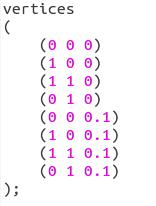
\includegraphics[scale=0.66]{vertices.png}
\caption{Coordinates of boundary geomtery points of the lid driven cavity}
\label{vertices}
\end{center}  
\end{figure}

\flushleft Then type block, inside which you can give the details of the boundary co-ordinates along with the number of mesh divisions in X, Y and Z direction in the following way$:$

\begin{figure}[ht]  
\begin{center}  
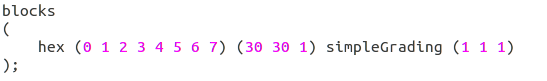
\includegraphics[scale=0.66]{blocks.png}
\caption{Block details of the geomtery}
\label{blocks}
\end{center}  
\end{figure}

\flushleft Here hex represents hexahedral block and the numbers inside first braces, next to that gives the names of the points at the boundary in clock-wise direction to form a block. Note that for more than one blocks the number of points would be more. The number of grid points can be modified as per requirement. For this problem we have used a 2-D mesh having 30x30 divisions and unit dept. Now since we have all straight edges in this geometry, we will keep the egdes empty.

\begin{figure}[ht]  
\begin{center}  
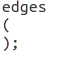
\includegraphics[scale=0.66]{edges.png}
\caption{edge details of the geomtery}
\label{edges}
\end{center}  
\end{figure}


\flushleft Next we give the details of the boundary conditions of the geometry. In this current problem we can see the following boundary conditions as shown below.

\begin{itemize}
  \item moving wall
  \item fixed wall
  \item front and back
\end{itemize}

\begin{figure}[ht]  
\begin{center}  
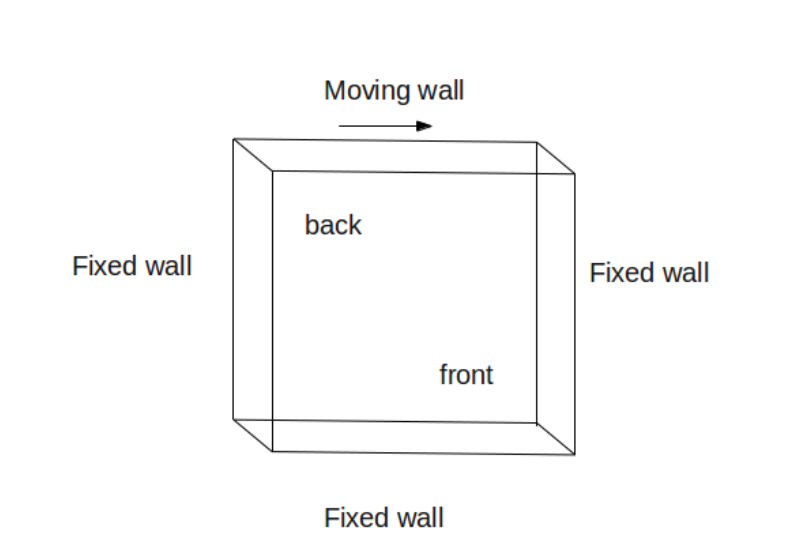
\includegraphics[scale=0.45]{boundary.png}
\caption{Boundary names of the lid driven cavity problem}
\label{boundary1}
\end{center}  
\end{figure}

\flushleft where it has a  moving wall at theb top and three fixed wall. The front and back faces are kept empty as this is a 2-D problem. Now in the blockMeshDict file you can type the boundary as following$:$

\begin{figure}[ht]  
\begin{center}  
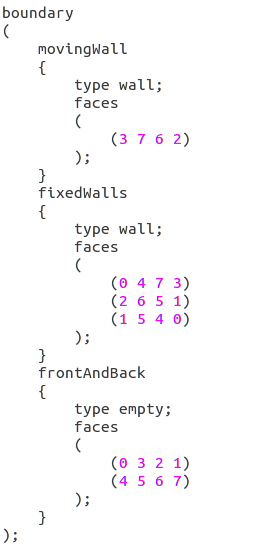
\includegraphics[scale=0.66]{boundary_name.png}
\caption{boundary details of the geomtery}
\label{boundary_name}
\end{center}  
\end{figure}


\flushleft Here within the boundary names enter the type of boundary you wish to use and  then faces, giving the points of the block forming a particular boundary. Note that you should be very careful while giving the order of the points. It should be given in such a way that if you place a folded palm on the surface of a boundary the thumb should be pointing normal to the surface and the fingers should be folded such that they make a curl in clockwise or anti-clockwise direction. Note that you should use either clockwise or anti-clockwise convention throughout the file and but not both at a time. Also you should be very careful regarding opening and closing of brackets in these files.
\flushleft After this, in a new line type mergePatchPairs. Since in this problem we do not have to merge any patches we will keep this empty as given below.

\begin{figure}[ht]  
\begin{center}  
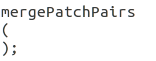
\includegraphics[scale=0.66]{merge.png}
\caption{merge patch details of the geomtery}
\label{merge}
\end{center}  
\end{figure}

\flushleft After completing writing  save it and close this file. Thus you have learned how to create a geomtery file.
\flushleft Now go back to the command terminal and type the following twice to go back to cavity folder:
\center \textbf{cd ..} 
\flushleft Next you can mesh this geomtry by typing blockMesh in the command terminal.This command would calculate the grid lines, number of cells, mesh details, etc for this particular geometry.

\flushleft\textbf{Post-Processing}
\flushleft  After this you can view the geometry by opening paraview. For this, type paraFoam in the command terminal and press $<$enter$>$.
\flushleft In the paraview window press Apply button on the left hand side(to include the geometry file in ParaFoam) of the Object Inspector Menu to view the Geometry, as shown in the Fig \ref{paraview1} $:$

\begin{figure}[ht]  
\begin{center}  
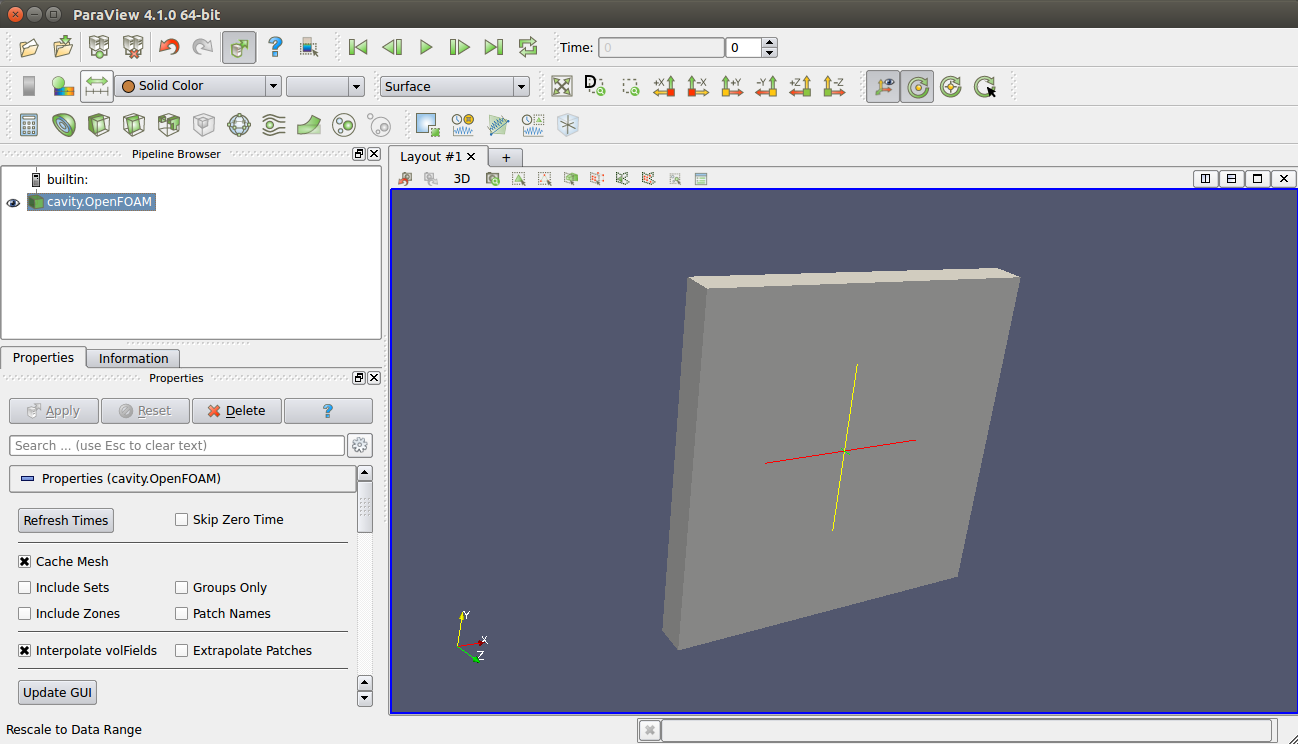
\includegraphics[scale=0.32]{paraview1.png}
\caption{Paraview window showing the 2-D geometry}
\label{paraview1}
\end{center}  
\end{figure}

\flushleft As you have learned in the previous chapter, you can use different feature in the paraview window to check the details of the geometry.


\end{document}
